\documentclass[12p]{article}
\usepackage[margin=1in, headheight=110pt]{geometry}
\usepackage{amssymb, amsmath, amsfonts, amsthm}
\usepackage{mathpazo}
\usepackage{setspace}
% \usepackage{probsoln}
\usepackage{fancyhdr}
\usepackage{hyperref}
\usepackage{float}
\usepackage{tikz}
\usepackage{enumitem}
\usepackage{graphicx}
\usepackage{listings}
\usepackage{caption}
\usepackage{bookmark}

\def\ojoin{\setbox0=\hbox{$\bowtie$}%
  \rule[-.02ex]{.25em}{.4pt}\llap{\rule[\ht0]{.25em}{.4pt}}}
\def\leftouterjoin{\mathbin{\ojoin\mkern-5.8mu\bowtie}}
\def\rightouterjoin{\mathbin{\bowtie\mkern-5.8mu\ojoin}}
\def\fullouterjoin{\mathbin{\ojoin\mkern-5.8mu\bowtie\mkern-5.8mu\o}}

\pagestyle{fancy}
\lhead{Evan Quan, Irene Chan, Patrick Gharib}
\rhead{SENG 300 - Group Project Iteration 1 - Winter 2018}
\title{\vspace{-6ex}Groupd Project Iteration 1}
\date{\vspace{-12ex}}


\newcommand{\code}[1]{\texttt{#1}}

\setlength{\parindent}{0pt}
\begin{document}
% \maketitle
\thispagestyle{fancy}

\begin{titlepage}
  \begin{center}
    \vspace{1cm}
    \Large{\textbf{University of Calgary}}\\
    \Large{\textbf{SENG 300  - Introduction to Software Engineering}}
    \vfill
    \line(1,0){400}\\[1mm]
    \huge{Group Project Iteration 1}\\
    \large{Finding Declarations and References}\\
    \line(1,0){400}\\
    \Large March 14, 2018\\
    \vfill
    \large{Evan Quan 10154242, Irene Chan 10103807, Patrick Gharib 10137116}\\
  \end{center}
\end{titlepage}

% \tableofcontents
% \thispagestyle{empty}
% \clearpage
%
% \onehalfspacing
%
% \setcounter{page}{1}

\section{Structural Diagram}
\begin{figure}[H]
  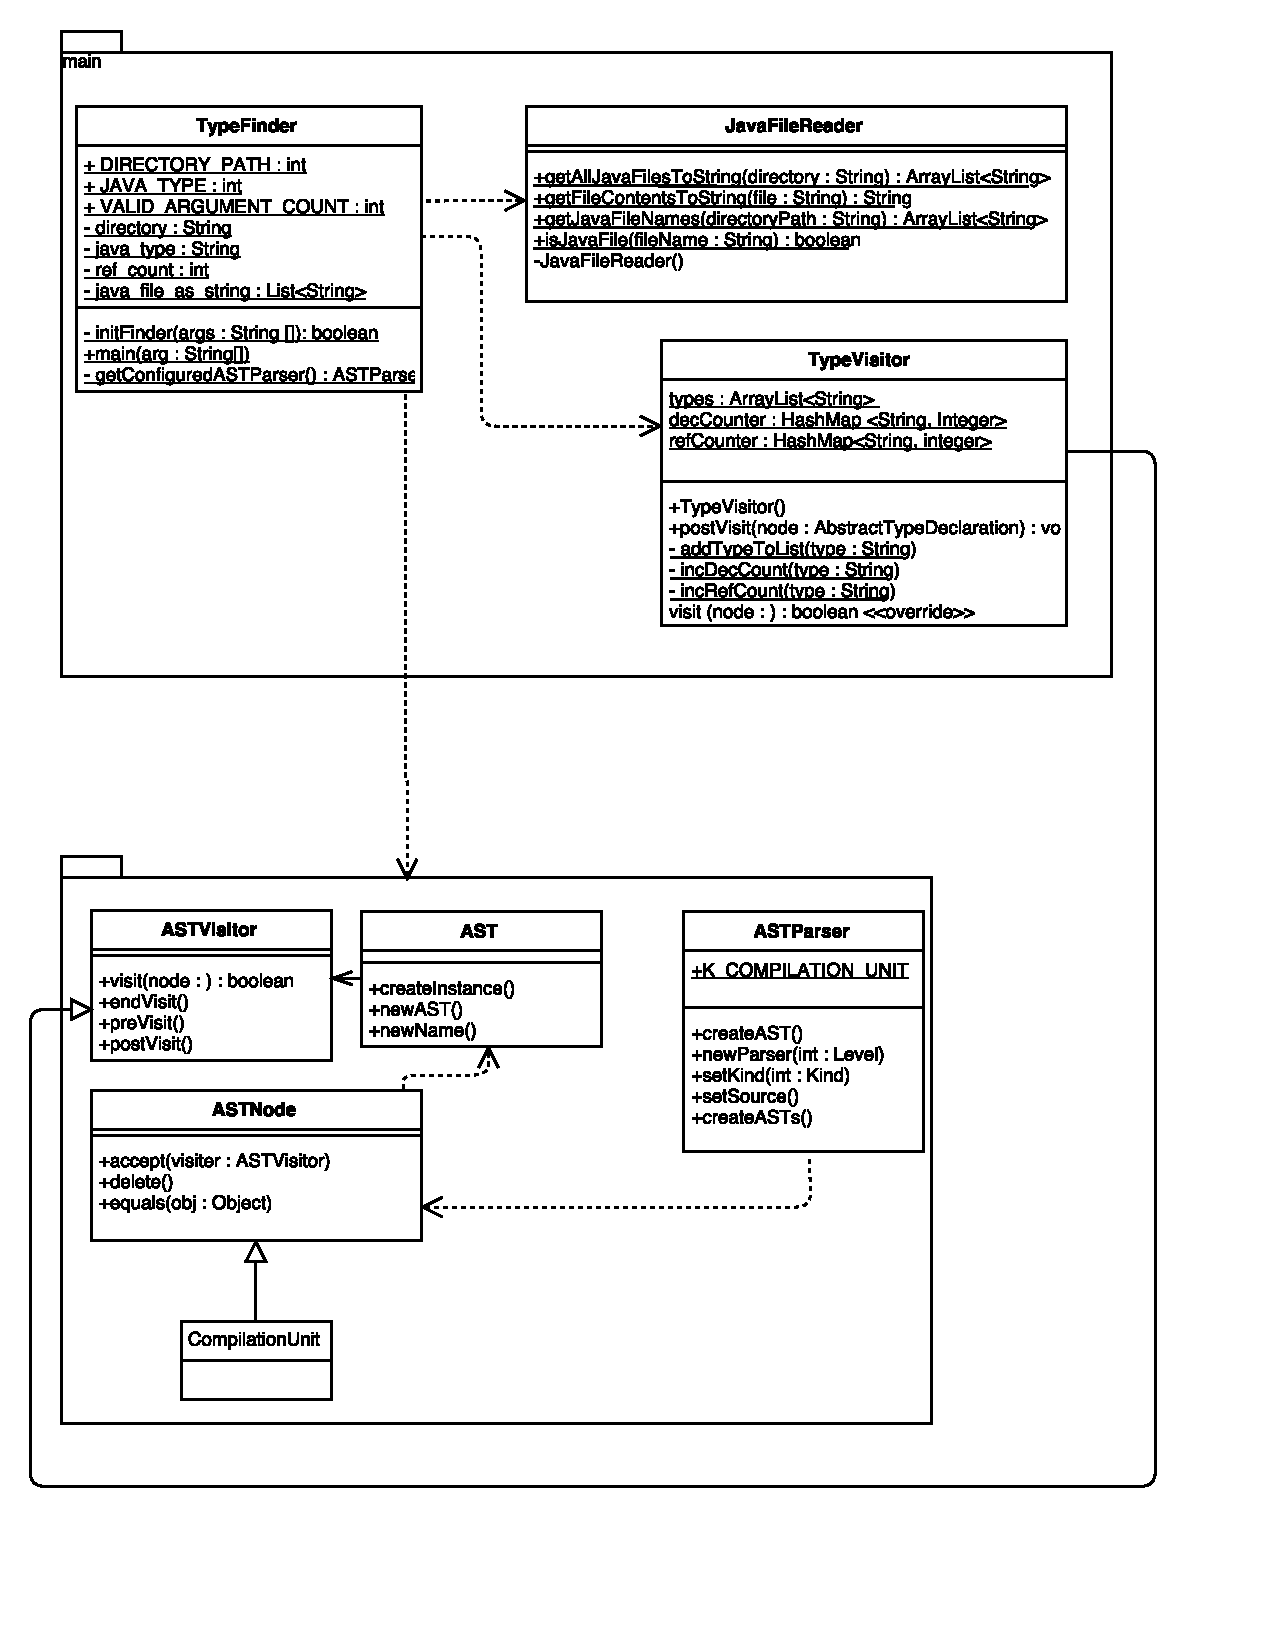
\includegraphics[width=0.95\textwidth]{SengUml.pdf}
  \caption{The relationship between our main package and relevant classes provided by org.eclipse.jdt.core.dom} % TODO caption
  \label{fig:structural}
\end{figure}


\section{Sequence Diagrams}
\begin{figure}[H]
  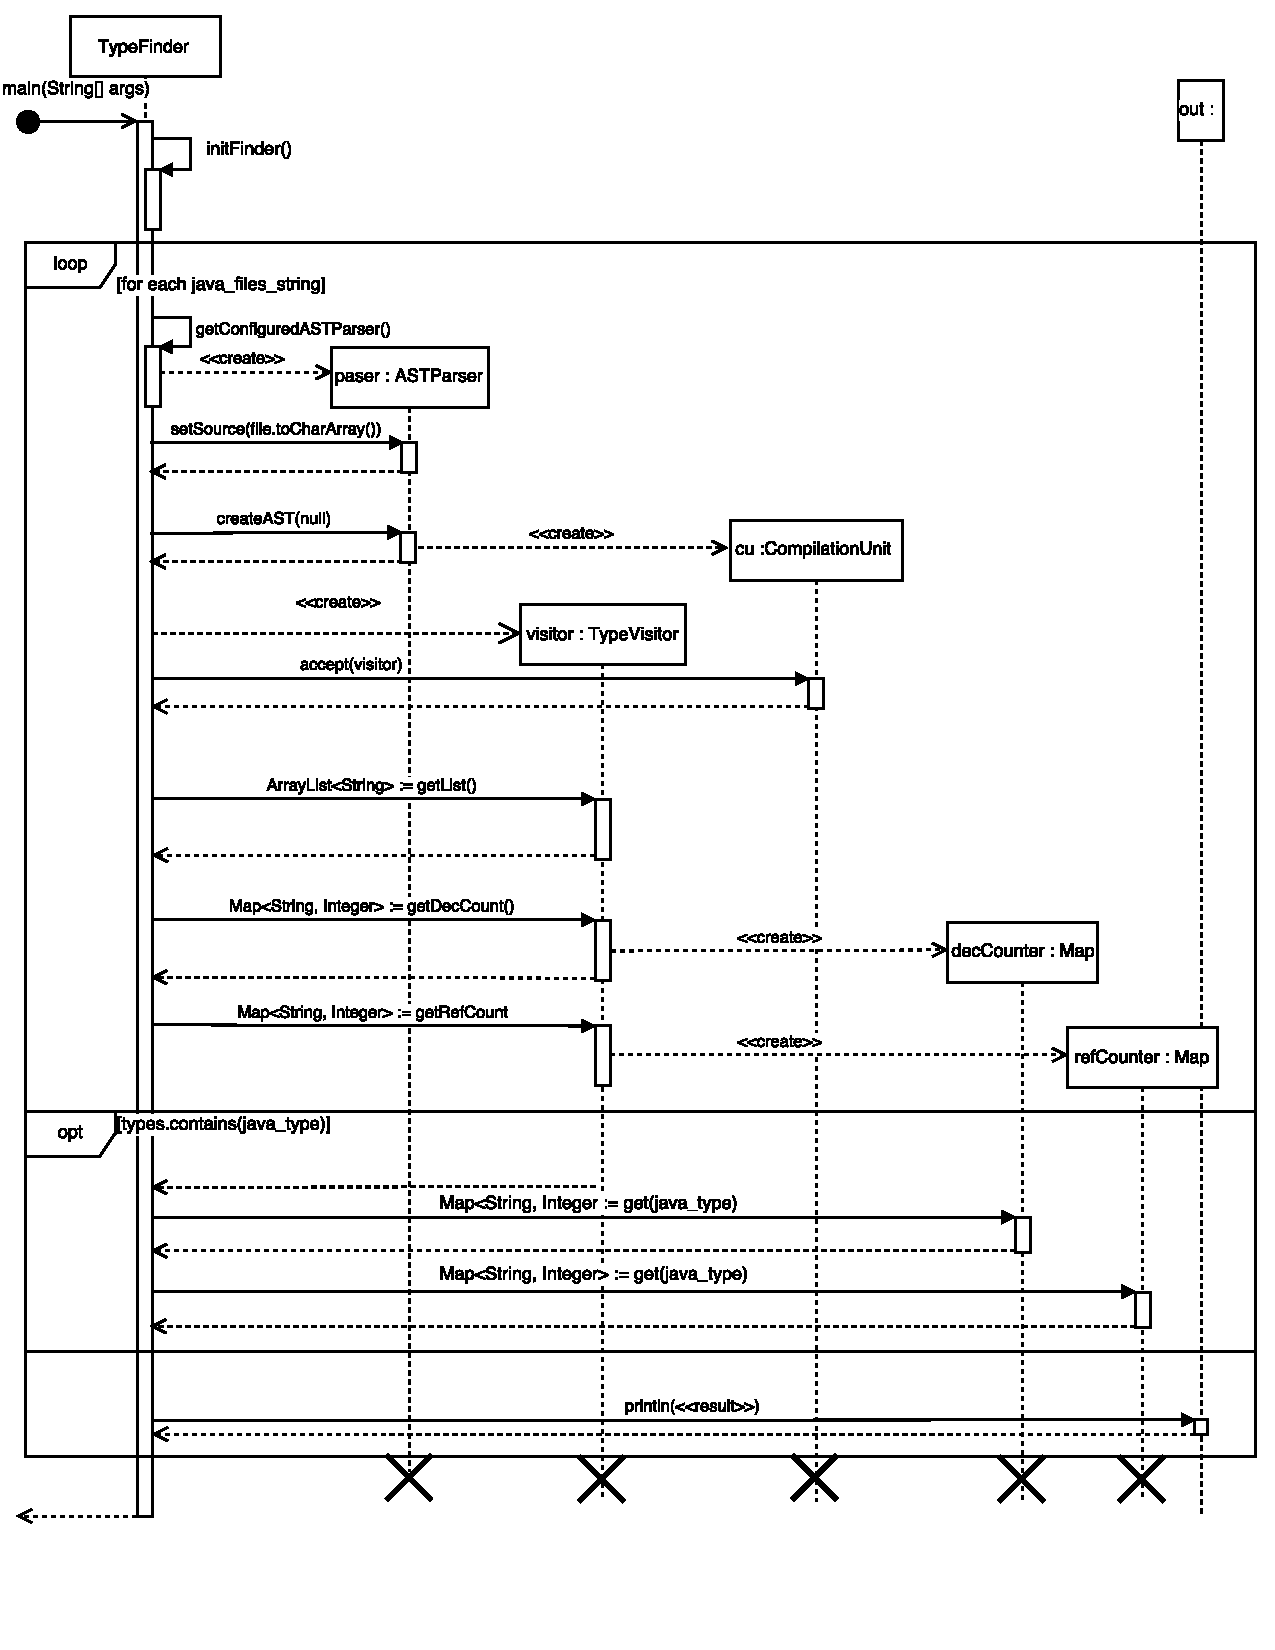
\includegraphics[width=0.95\textwidth]{mainTypeFinder.pdf}
  \caption{Sequence of TypeFinder program intialization and completion} % TODO caption
  \label{fig:sequence1}
\end{figure}

\begin{figure}
  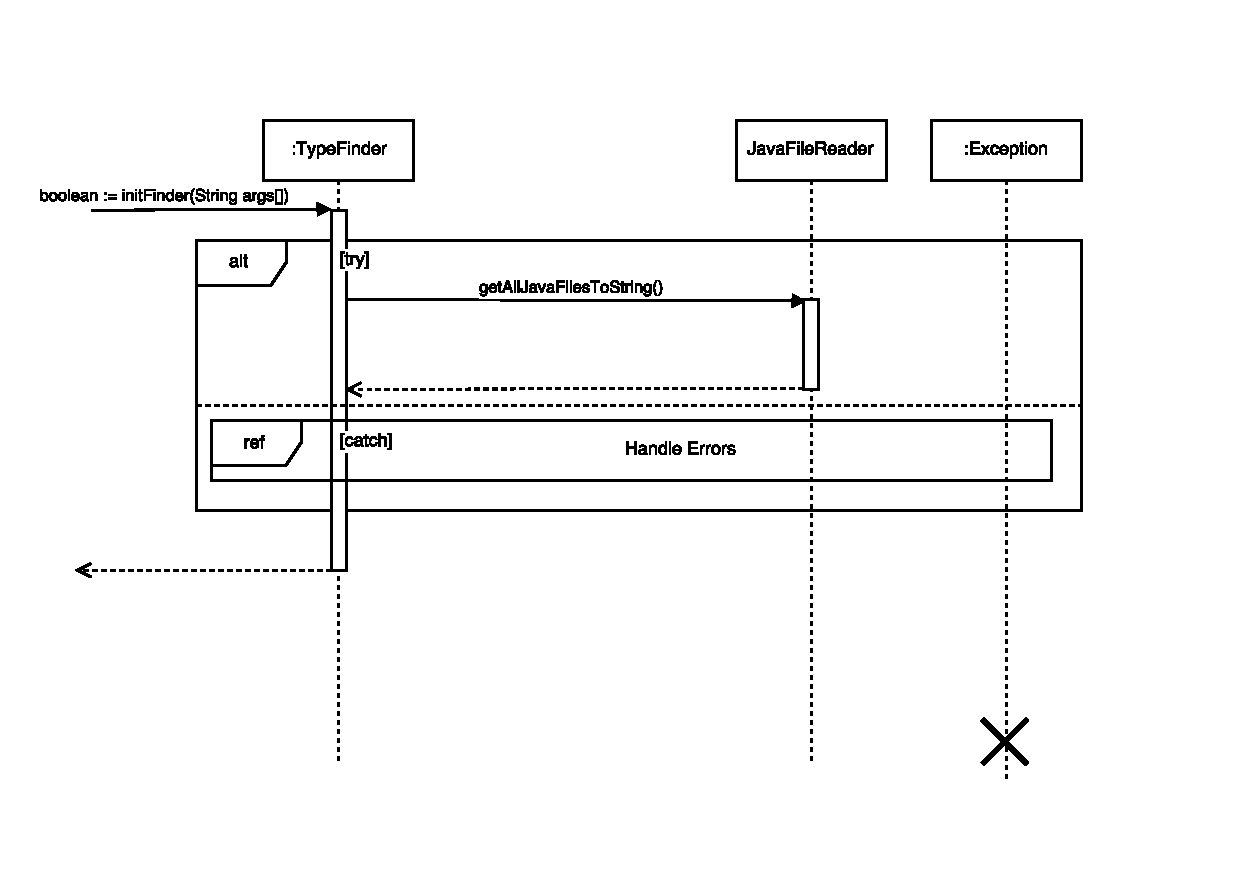
\includegraphics[width=1.0\textwidth]{initFrinder.pdf}
  \caption{Initializing TypeFinder involving checking for valid user input. If valid, it acqures the Java file contents and setting up the information necessary for parsing. If invalid, prompt the user with an error message.} % TODO caption
  \label{fig:sequence2}
\end{figure}

\begin{figure}
  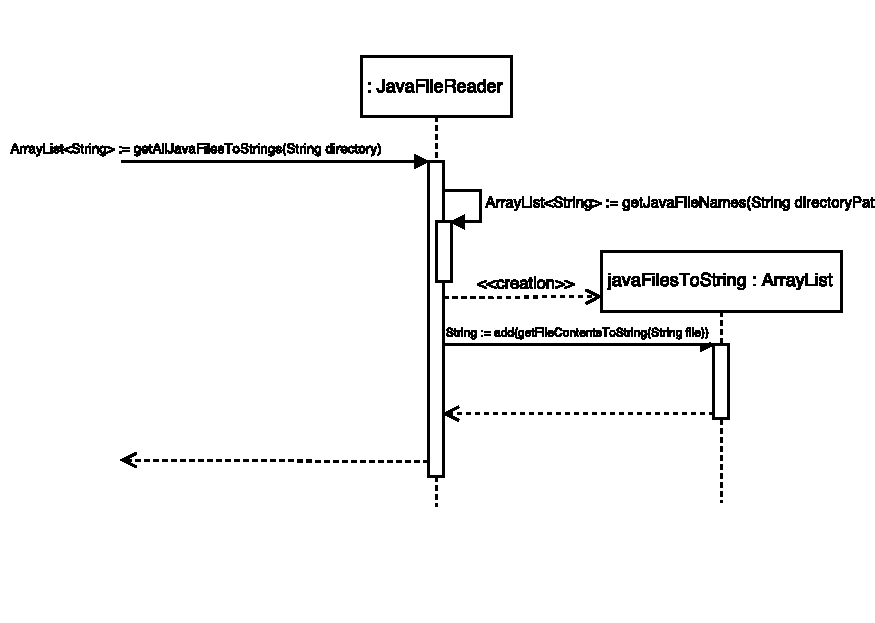
\includegraphics[width=1.0\textwidth]{getAllJavaFilesToString.pdf}
  \caption{JavaFileReader retrieves the contents of all Java files in a directory, one file at a time.} % TODO caption
  \label{fig:sequence2}
\end{figure}

\newpage

\section{State Diagram}
\begin{figure}[H]
  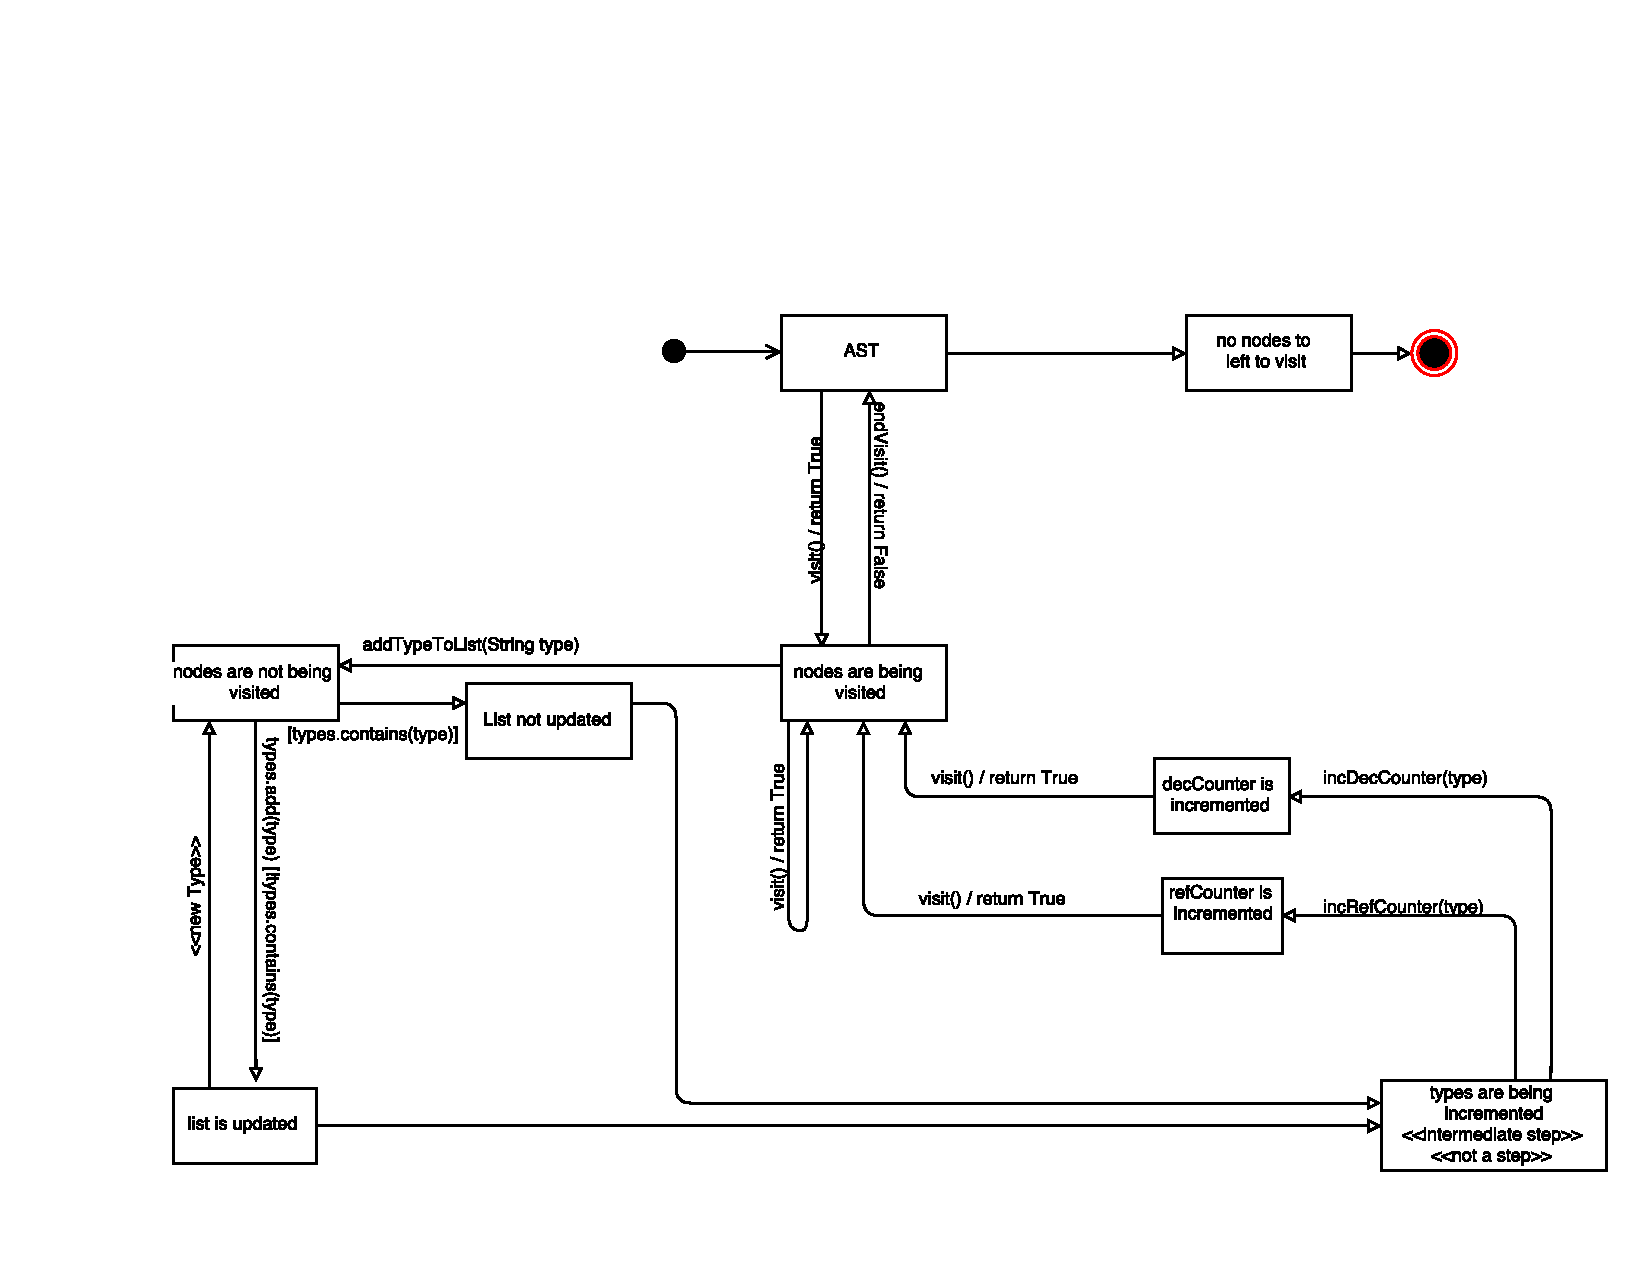
\includegraphics[width=1.0\textwidth]{State_diagram.pdf}
  \caption{The state of the program in finding declaration and reference counts.} % TODO caption
  \label{fig:state}
\end{figure}

\newpage
\onehalfspacing
\section{Explanation}

\subsection{Usage}
Run the Java \code{TypeFinder.class} file through command line:

\code{java TypeFinder <directory> <Java type>}

\code{directory} is the path of the directory (either absolute or relative).

\subsection{Struture}
The UML diagram was kept as simple as possible and only represent main components of the software. All the methods in the Type Finder Class were included since they drive the software during execution. The JavaFileReader class is reads the all files in the directory and allows for parsing via AST. We Did not include all the methods for the TypeVisitor. The abstracted details were only supporting features that did not aid in the understanding of the functionality. As for visit(node : ) : boolean, the formating was done this way due to the multiple overriden methods with different parameter types, such as SingleVariableDecleration, TypeDecleration...etc.
like the rest only the key components of  the ASTParser, AST, ASTVistor, ASTNode were maintained in the uml Diagram. Everything that did not aid or was none essential in understanding the relationships between the TypeFinder and the AST parser was left out.

\subsection{Sequence}
The software works by recieving arguments from the user, those being the directory of interest and the fully qualified name of a java type. It the enters a loop which executes per file read. After entering the loop, the ASTParser is configured with the correct specifications  and created. after that the the file to be read is set and the AST is created along with a visitor. we then begin to visit the nodes of the ast count the number of decleration/references of types. finally at the end of the loop we sum the total number of counts. the loop is exited and the number of references and declerations in printed to the console.

The inner workings of the getConfiguredASTParser() method is non-essential to the client's understanding of the software. Thus the details were abstracted away and not expanded on. Another aspect of the code that was abstracted away was most of the methods in JavaFileReader. We modeled a very broad overview, this informs anyone viewing the model (provided some basic knowledge of java) of what is happening. Had we made our diagram anymore specific in this area, it would draw attention away from the more important functionality of the software, and would only overwhelm the viewer. A very basic diagram shows the execution of initFinder, which was only meant to serve the purpose of showing that the javaFileReader Class was being used to read the files. A more Specific sequence diagram was provided to show how getAllJavaFilesToStrings() was recieving information about the directory and files, as well as how it returned the rusult for ASTParser to use.

\end{document}
